\documentclass{examen}

\begin{document}
\modulo{Lenguajes de marcas y sistemas de gesti�n de informaci�n}


\pregunta{En el HTML siguiente se genera un formulario con tres controles
\begin{itemize}
\item{El primer control se llama ``num1'' y siempre es un n�mero entero}
\item{El segundo control es una lista desplegable y el usuario puede seleccionar dos opciones llamadas ``sumar'' y ``restar''.}
\item{El tercer control se llama ``num2'' y siempre es un n�mero entero}
\end{itemize}
Crear una aplicaci�n que en funci�n de la operaci�n que elija el usuario muestre la suma o la resta de los dos n�meros. Observa que hay
un boton que al ser pulsado llama a la funci�n {\tt calcular()}
}{3.5}

\begin{verbatim}
<form>
    <input type="text" id="num1">
    <select id="operacion">
        <option value="sumar">+</option>
        <option value="restar">-</option>
    </select>
    <input type="text" id="num2">
	<input type="submit" onclick="calcular();return false;">
</form>

\end{verbatim}

\break

\pregunta{Una editorial desea ofrecer a sus clientes una aplicaci�n que les permita saber como combinar la compra de sus peri�dicos y revistas de la forma que les resulte m�s ventajosa. 

Las revistas se llaman TodoCiencia, SoloTV y MasCrucigramas y los precios de sus suscripciones son respectivamente son 100, 50 y 40 euros anuales. Los peri�dicos ``El diario'', ``El suceso'' y ``Econoticias'' cuestan respectivamente 200, 180 y 150 euros anuales. Se puede combinar una revista con uno o m�s peri�dicos. Por defecto debe aparecer marcada la revista ``TodoCiencia`` con todos los peri�dicos marcados.

La editorial anterior desea que la aplicaci�n anterior implemente ciertos comportamientos en funci�n de las ofertas:

\begin{itemize}
\item{ Cuando el cliente marque revistas o peri�dicos la aplicaci�n mostrar� en el recuadro las publicaciones que el usuario compra as� como el precio total a pagar.}
\item{ Si se marca un peri�dico cualquiera y una revista el precio total se reduce al 90\%.}
\item{ Observa que hay
un boton que al ser pulsado llama a la funci�n {\tt calcular()}}
\end{itemize}
}{6.5}

\begin{figure}[h]
\centering
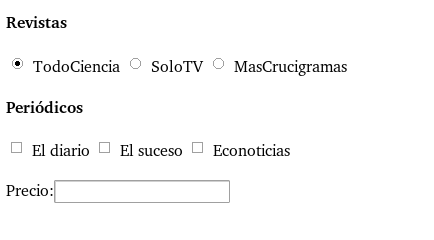
\includegraphics[width=.8\textwidth]{examen-img/revistas.png}
\caption{Formulario de compra editorial}
\end{figure}

\break

\begin{verbatim}
<!-- HTML con los controles-->
<h4>Revistas</h4>
<input type="radio" name="revistas" value="ciencia" id="ciencia" checked>

<label for="ciencia">TodoCiencia</label>
<input type="radio" name="revistas" value="tv" id="tv">

<label for="tv">SoloTV</label>
<input type="radio" name="revistas" value="crucigramas" id="crucigramas">
                   
<label for="crucigramas">MasCrucigramas</label>

<h4>Peri�dicos</h4>

<input type="checkbox" name="periodicos[]" id="diario" value="diario" >
<label for="diario">El diario</label>
                    
<input type="checkbox" name="periodicos[]" id="suceso" value="suceso">
<label for="suceso">El suceso</label>
                    
<input type="checkbox" name="periodicos[]" id="econoticias" value="econoticias">
<label for="econoticias">Econoticias</label>

Precio:<input type="text" id="precio_total"> 
<input type="submit" onclick="calcular();return false;">
\end{verbatim}
\end{document}
